\section{Simplifcation Rules}

In the previous section we saw how we can calculate the matrix-representation of a ZX-diagram. But the way we used to evaluate the circuit was very inefficient. We had to calculate the matrix-representation of every single spider and had to perform heavy matrix multiplications and tensor products. This is exactly the same process as if we had just calculated the circuit using the classical logic gate model. So we did not gain anything from using the ZX-diagram. In this section we will look at a set of rewrite rules which allow us to simplify ZX-diagrams by using rewrite rules.

Note that all the rules can be applied in both directions. This means that we can use the rules to simplify a diagram, but we can also use them to make a diagram more complex. Additionally, we can apply the rules to any subgraph of the diagram, provided that the shape of the subgraph matches the shape of the rule. It is also important to know that all the rules also hold if we replace all the spiders with their adjoint (I.e.we swap the color of $\mathbf{all}$ spiders).

We also don't have to keep track which leg of the spider is the input and which one is the output. This rule corresponds to the $\textit{Only topology matters}$ mantra we introduced in the previous section.

\subsection{Identity Removal}

The rule we will look at is the identity removal rule. It isn't actually a simplification rule, but it makes it way easier to remove clutter from the diagram. The rule states that we can remove any spider with exactly one input and one output if it has a phase of $0$, and can replace it with a single edge.
This rule is shown in figure \ref{fig:identity_removal_rule}.

\begin{figure}[h]
    \centering
    \begin{ZX}
        \rar & \zxZ{}   \rar &\\
    \end{ZX}=
    \begin{ZX}
        \rar  &\rar &\\
    \end{ZX}=
    \begin{ZX}
        \rar & \zxX{}   \rar &\\
    \end{ZX}
    \caption{Identity Removal Rule}
    \label{fig:identity_removal_rule}
\end{figure}



\subsection{Spider Fusion}

The spider fusion rule allows us to fuse two spiders together if they are connected by an edge. The inputs and outputs of the two spiders are merged together. Additionally the phase of the two spiders is added together.

This rule is shown in figure \ref{fig:spider_fusion_rule}.

\begin{figure}[h]
    \centering
    \begin{ZX}
        \leftManyDots{k}  \zxZ{\alpha} \ar[rd,o.]  \rightManyDots{l}\\
        \zxNone{} & \leftManyDots{n}  \zxZ{\beta}  \rightManyDots{m}
    \end{ZX} =
    \begin{ZX}
        \leftManyDots{k+n}  \zxZ{\alpha+\beta} \rightManyDots{l+m}
    \end{ZX}
    \caption{Spider Fusion Rule}
    \label{fig:spider_fusion_rule}
\end{figure}



\subsection{Hopf Rule}

The Hopf rule allows us to split apart two spiders of opposite color, given that they are connected by two edges.

This rule is shown in figure \ref{fig:hopf_rule}.

\begin{figure}[h]
    \centering
    \begin{ZX}
        \rar & \zxZ{\alpha} \ar[r,o.] \ar[r,o'] & \zxX{\beta} \rar &\\
    \end{ZX} =
    \begin{ZX}
        \rar & \zxZ{\alpha}  & \zxX{\beta} \rar &\\
    \end{ZX}
    \caption{Hopf Rule}
    \label{fig:hopf_rule}
\end{figure}

\subsection{Copy Rule}

The copy rule allows to copy the computational basis states through a spider of the opposite color. This rule corresponds to the $\textit{"Green copies Red"}$ / $\textit{"Red copies Green"}$ mantra. The copied state is then moved to $\mathbf{all}$ the outputs of the spider.

This rule is shown in figure \ref{fig:copy_rule}.

\begin{figure}[h]
    \centering
    \begin{ZX}
        & & \zxNone{} \\
        & & \zxNone{} \\
        \zxX{a \pi} \rar &  \zxZ{\alpha}  \rar \ar[ruu,s] \ar[rdd,s] & \\
        & & \zxNone{} \\
        & & \zxNone{} \\
    \end{ZX} =
    \begin{ZX}
        \zxX{a \pi} \rar &\\
        \zxX{a \pi} \rar &\\
        \zxX{a \pi} \rar &\\
    \end{ZX}
    \caption{Copy Rule}
    \label{fig:copy_rule}
\end{figure}

Note that this rule only works when $a$ is $0$ or $1$, as we can only copy computational basis states as they are orthogonal to each other \cite{dave2006teleportation}. This means only $|0\rangle$, $|1\rangle$, $|+\rangle$ and $|-\rangle$ can be copied using this rule.

\subsection{Bi-Algebra Rule}

The bi-algebra works as seen in figure \ref{fig:bi-algebra_rule}. It has an analogous rule in digital logic, where it states that the copied $\mathit{XOR}$ result, corresponds to first copying the inputs and then performing an $\mathit{XOR}$ on the swapped, and copied inputs. This rule is shown in figure \ref{fig:fig:bi-algebra_rule-digital}. It works by using the copy-rule from figure \ref{fig:copy_rule} and a $\mathit{XOR}$ spider.

\begin{figure}[h]
    \centering

    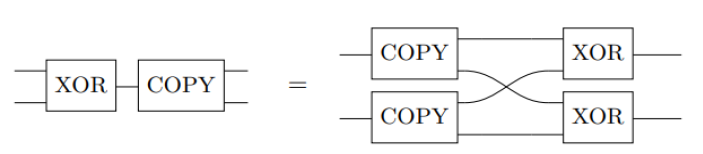
\includegraphics[width=8cm]{images/bi-algebra-rule-digital-logic.png}
    \caption{Bi-Algebra Rule in Digital Logic}
    \label{fig:fig:bi-algebra_rule-digital}
\end{figure}

\begin{figure}[h]
    \centering
    \begin{ZX}
        \zxNone{} \ar[rd,-N]  & & &\zxNone{}  \\
        &  \zxX{}  \rar & \zxZ{} \ar[ru,N-] \ar[rd,N-] \\
        \zxNone{} \ar[ru,-N] & & &\zxNone{}  \\
    \end{ZX} =
    \begin{ZX}
        \rar& \zxZ{} \rar \ar[rd] & \zxX{} \rar &\\
        \rar& \zxZ{} \rar \ar[ru] & \zxX{} \rar &\\
    \end{ZX}
    \caption{Bi-Algebra Rule}
    \label{fig:bi-algebra_rule}
\end{figure}


\subsection{$\pi$-Commutation Rule}

The $\pi$-commutation rule allows us to move a spider with phase $\pi$ through a spider of the opposite color. By moving the spider through the other spider, the phase of the spider is inverted. This rule is shown in figure \ref{fig:pi-commutation_rule}.

\begin{figure}[h]
    \centering
    \begin{ZX}
        & && \zxNone{} \\
        & && \zxNone{} \\
        \rar &  \zxX{\pi} \rar &  \zxZ{\alpha}  \rar \ar[ruu,s] \ar[rdd,s] & \\
        & && \zxNone{} \\
        & && \zxNone{} \\
    \end{ZX} =
    \begin{ZX}
        & & \zxX{\pi} \\
        \rar &  \zxZ{-\alpha}  \rar \ar[ru,s] \ar[rd,s] &\zxX{\pi} \\
        & & \zxX{\pi} \\
    \end{ZX}
    \caption{$\pi$-Commutation Rule}
    \label{fig:pi-commutation_rule}
\end{figure}

\subsection{Color Change Rule}

The color change rule allows us to change the color of a spider. This is done by adding a $\mathit{H}$ gates to all the inputs and outputs of the spider. This rule is shown in figure \ref{fig:color_change_rule}.


\begin{figure}[h]
    \centering
    \begin{ZX}
        \zxN{} \ar[rd,edge above,-N.,end anchor=180-45] &[\zxwCol,\zxHCol] &[\zxwCol,\zxHCol] \zxN{} \\[\zxNRow]%%
        & \zxZ{\alpha}
        \ar[ru,N'-,start anchor=45]
        \ar[rd,N.-,start anchor=-45] & \\[\zxNRow]
        \zxN{} \ar[ru,-N',end anchor=180+45] & & \zxN{}
    \end{ZX}
    \begin{ZX}
        \zxN{} \ar[rd,edge above,-N.,H,end anchor=180-45] &[\zxwCol,\zxHCol] &[\zxwCol,\zxHCol] \zxN{} \\[\zxNRow]%%
        & \zxX{\alpha}
        \ar[ru,N'-,H,start anchor=45]
        \ar[rd,N.-,H,start anchor=-45] & \\[\zxNRow]
        \zxN{} \ar[ru,-N',H,end anchor=180+45] & & \zxN{}
    \end{ZX}
    \caption{Color Change Rule}
    \label{fig:color_change_rule}
\end{figure}

Where a Hadamard gate is defined in figure \ref{fig:hadamard_gate}. Note that we use the decomposition of the Hadamard gate into three sequential $\frac{\pi}{2}$ rotations to represent the Hadamard gate in the ZX-calculus.

\begin{figure}[h]
    \centering
    \begin{ZX}
        \zxN{} \rar &[\zxwCol] \zxH{} \rar &[\zxwCol] \zxN{}
    \end{ZX}
    =
    \begin{ZX}
        \rar &\zxZ{\frac{\pi}{2}} \rar & \zxX{\frac{\pi}{2}}  \rar & \zxZ{\frac{\pi}{2}} \rar & \\
    \end{ZX}
    \caption{Hadamard Gate}
    \label{fig:hadamard_gate}
\end{figure}


